% !TeX spellcheck = en_US

\chapter{Theoretical and Practical Challenges}

\section{Building outline regularization}
Once the network has been trained, it can be used to make predictions on images, it has never "seen" before. However, there are situations in which the predictions are far from perfect, especially then if the building is partially covered from trees or has unclear outlines. This can be seen in \autoref{fig:challenges:building_masks}.

\begin{figure}[H]
	\centering
	\begin{subfigure}{0.4\textwidth}
		\centering
    	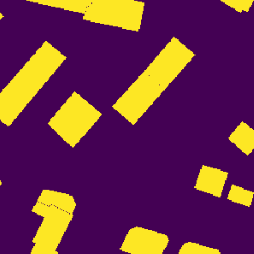
\includegraphics[width=0.9\linewidth]{chapters/challenges/images/predicted_masks_gt.png}		    \caption{Actual ground truth}
    	\label{fig:challenges:predicted_building_masks_gt}
	\end{subfigure}~
		\begin{subfigure}{0.4\textwidth}
		\centering
    	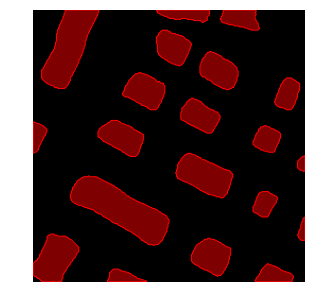
\includegraphics[width=0.9\linewidth]{chapters/challenges/images/predicted_masks.png}		    \caption{Predicted building masks}
    	\label{fig:challenges:predicted_building_masks}
	\end{subfigure}
	\caption{Predicted masks and actual ground truth}
	\label{fig:challenges:building_masks}
\end{figure}

As a result of the inaccuracies in the predicted building masks the contours of these predictions can not directly be used to create the vectorized outlines. Instead, the predictions have to be regularized. The approach used is similar to \cite{Partovi.2017} and described in \autoref{fig:challenges:rectangularization}.

\begin{figure}[H]
\centering
\begin{tikzpicture}[node distance = 2cm, auto, scale=0.7, every node/.style={transform shape}]
    % Place nodes
    \node [cloud] (mask) {Predicted mask};
    \node [block, below of=mask] (extract_contour) {Extract contour};
    \node [cloud, below of=extract_contour] (contour) {Approximated contour};
    \node [block, below of=contour] (segment) {Line segmentation};
    \node [cloud, below of=segment] (line_segments) {Line segments};
    \node [block, below of=line_segments] (assign_orientation) {Create orientation classes};
    \node [block, below of=assign_orientation] (assign_neighbourhoods) {Create neighbourhoods};
    \node [block, below of=assign_neighbourhoods] (rotate_lines) {Rotate lines};
    \node [block, below of=rotate_lines] (get_corner_points) {Get corner points};
    \node [cloud, below of=get_corner_points] (corner_points) {Building corner points};

    % Draw edges
    \path [line,dashed] (mask) -- (extract_contour);
    \path [line,dashed] (extract_contour) -- (contour);
    \path [line,dashed] (contour) -- (segment);
    \path [line,dashed] (segment) -- (line_segments);
    \path [line,dashed] (line_segments) -- (assign_orientation);
    \path [line] (assign_orientation) -- (assign_neighbourhoods);
    \path [line] (assign_neighbourhoods) -- (rotate_lines);
    \path [line] (rotate_lines) -- (get_corner_points);
    \path [line,dashed] (get_corner_points) -- (corner_points);
\end{tikzpicture}
	\caption{Rectangularization procedure}
	\label{fig:challenges:rectangularization}
\end{figure}

The single steps are described in detail in the following sections.

\begin{figure}[H]
    \centering
	\begin{subfigure}{0.4\textwidth}
    	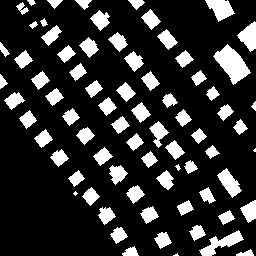
\includegraphics[width=0.9\linewidth]{chapters/challenges/images/regular_building_masks.png}		    \caption{Regular buildings}
    	\label{fig:challenges:regular_buildings}
	\end{subfigure}~
	\begin{subfigure}{0.4\textwidth}
    	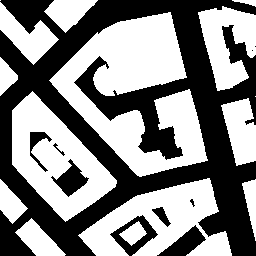
\includegraphics[width=0.9\linewidth]{chapters/challenges/images/irregular_building_masks.png}       	\caption{Non-orthogonal buildings}
    	\label{fig:challenges:irregular_buildings}
	\end{subfigure}
	\caption{Different kinds of buildings with regard to their corner angles}
	\label{fig:challenges:building_masks}
\end{figure}

\subsection{Contour extraction}
The first step of the building outline regularization procedure consists of getting the contour from the predicted mask, which covers the whole building. The extraction is done using the marching squares algorithm \cite{Maple.2003}. In this algorithm, a square consisting of four cells is moved (marched) along the contour in such a way, that at least one cell always covers the object to be contoured. Additionally, the square always has a state, which is derived from the content of its cells, according to \eqref{equ:challenges:marching_squares_state}. The cells are traversed in counter clockwise order.

\newenvironment{conditions}
  {\par\vspace{\abovedisplayskip}\noindent\begin{tabular}{>{$}l<{$} @{${}={}$} l}}
  {\end{tabular}\par\vspace{\belowdisplayskip}}

\begin{equation}
\begin{split}
	s	&= \displaystyle\sum_{i=0}^3 2^i f(c_i) \\
		&= 2^0 * f(c_0) + 2^1 * f(c_1) + 2^2 * f(c_2) + 2^3 * f(c_3) \\
		&= f(c_{bottomLeft}) + 2 * f(c_{bottomRight}) + 4 * f(c_{topRight}) + 8 * f(c_{topLeft})
	\label{equ:challenges:marching_squares_state}
\end{split}
\end{equation}
where:
\begin{itemize}[label=]
    \item $c_i$: The value of the cell $i$
    \item $c_0$: The bottom left cell
\end{itemize}

and

\[ f(c_i) =
  \begin{cases}
    0  & \text{if $c_i \leq 0$}\\
    1  & \text{if $c_i > 0$}
  \end{cases}
\]


As soon as the contour has been extracted, its number of points will be reduced using a Douglas-Peucker algorithm \cite{DOUGLAS.1973}. The reason for this is, that the contour has pixel accuracy. That means, there may be several points on the same horizontal or vertical line, even though, the startpoint and endpoint of each such line would be enough, to represent the line. Additionally, the lower the number of points per contour is, the faster the following processing will be.

\begin{figure}[H]
    \centering
	\begin{subfigure}{0.4\textwidth}
    	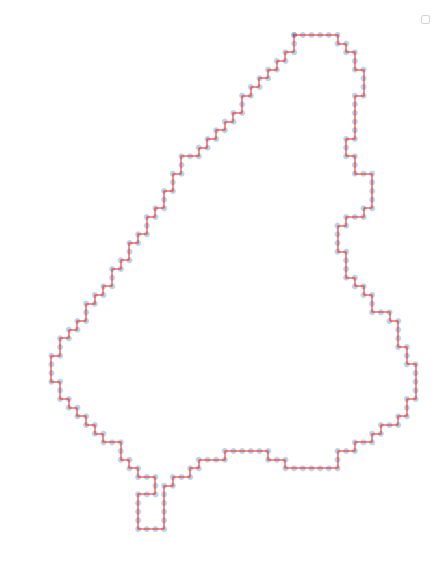
\includegraphics[width=0.9\linewidth]{chapters/challenges/images/original_contour.png}		    	\caption{Original contour}
	\end{subfigure}~
	\begin{subfigure}{0.4\textwidth}
    	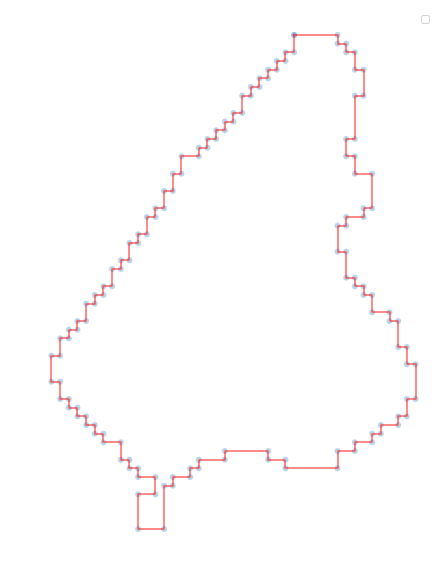
\includegraphics[width=0.9\linewidth]{chapters/challenges/images/approx_contour.png}       			\caption{Approximated contour}
	\end{subfigure}
	\caption{Contour before and after approximation}
	\label{fig:challenges:contour_approximation}
\end{figure}

\subsection{Line segmentation}
Once the contour has been extracted, it is split into multiple line segments. For this, the main direction of the building is determined using the Hough lines algorithm. The result of this is the line which hits the greatest number of points. The angle between this line and a horizontal line gives the main building orientation.

Once the main building direction is known, the line segmentation starts at the point which has the smallest distance to this line. The following algorithm describes the line segmentation process.

\begin{algorithm}[H]
\KwData{Contour points, startpoint}
\KwResult{Lines}
rearrange points so that startpoint == points[0]
lines = []
\While{any points left}{
	segment = remove first 3 elements from points
	\While{points is not empty}{
		p = points.first()
		err = rsme of distance between segment.last() and p
		\If{err > threshold}{
			break
		}
		
		segment.append(p)
		points.remove(p)
	}
	\If{segment.length() >= 3}{
		line = fit line to points of segment
		lines.append(line)
	}
}
\caption{Line segmentation algorithm}
\end{algorithm}

	
\subsection{Create orientation classes}
tbd

\subsection{Create neighbourhoods}
tbd

\subsection{Update line orientation}
tbd

\subsection{Get corner points}
tbd